\documentclass[]{article}
\usepackage{lmodern}
\usepackage{amssymb,amsmath}
\usepackage{ifxetex,ifluatex}
\usepackage{fixltx2e} % provides \textsubscript
\ifnum 0\ifxetex 1\fi\ifluatex 1\fi=0 % if pdftex
  \usepackage[T1]{fontenc}
  \usepackage[utf8]{inputenc}
\else % if luatex or xelatex
  \ifxetex
    \usepackage{mathspec}
  \else
    \usepackage{fontspec}
  \fi
  \defaultfontfeatures{Ligatures=TeX,Scale=MatchLowercase}
\fi
% use upquote if available, for straight quotes in verbatim environments
\IfFileExists{upquote.sty}{\usepackage{upquote}}{}
% use microtype if available
\IfFileExists{microtype.sty}{%
\usepackage{microtype}
\UseMicrotypeSet[protrusion]{basicmath} % disable protrusion for tt fonts
}{}
\usepackage[margin=1in]{geometry}
\usepackage{hyperref}
\hypersetup{unicode=true,
            pdftitle={Locker-Angelina-ADA-Homework-02},
            pdfauthor={Angelina Locker},
            pdfborder={0 0 0},
            breaklinks=true}
\urlstyle{same}  % don't use monospace font for urls
\usepackage{color}
\usepackage{fancyvrb}
\newcommand{\VerbBar}{|}
\newcommand{\VERB}{\Verb[commandchars=\\\{\}]}
\DefineVerbatimEnvironment{Highlighting}{Verbatim}{commandchars=\\\{\}}
% Add ',fontsize=\small' for more characters per line
\usepackage{framed}
\definecolor{shadecolor}{RGB}{248,248,248}
\newenvironment{Shaded}{\begin{snugshade}}{\end{snugshade}}
\newcommand{\KeywordTok}[1]{\textcolor[rgb]{0.13,0.29,0.53}{\textbf{#1}}}
\newcommand{\DataTypeTok}[1]{\textcolor[rgb]{0.13,0.29,0.53}{#1}}
\newcommand{\DecValTok}[1]{\textcolor[rgb]{0.00,0.00,0.81}{#1}}
\newcommand{\BaseNTok}[1]{\textcolor[rgb]{0.00,0.00,0.81}{#1}}
\newcommand{\FloatTok}[1]{\textcolor[rgb]{0.00,0.00,0.81}{#1}}
\newcommand{\ConstantTok}[1]{\textcolor[rgb]{0.00,0.00,0.00}{#1}}
\newcommand{\CharTok}[1]{\textcolor[rgb]{0.31,0.60,0.02}{#1}}
\newcommand{\SpecialCharTok}[1]{\textcolor[rgb]{0.00,0.00,0.00}{#1}}
\newcommand{\StringTok}[1]{\textcolor[rgb]{0.31,0.60,0.02}{#1}}
\newcommand{\VerbatimStringTok}[1]{\textcolor[rgb]{0.31,0.60,0.02}{#1}}
\newcommand{\SpecialStringTok}[1]{\textcolor[rgb]{0.31,0.60,0.02}{#1}}
\newcommand{\ImportTok}[1]{#1}
\newcommand{\CommentTok}[1]{\textcolor[rgb]{0.56,0.35,0.01}{\textit{#1}}}
\newcommand{\DocumentationTok}[1]{\textcolor[rgb]{0.56,0.35,0.01}{\textbf{\textit{#1}}}}
\newcommand{\AnnotationTok}[1]{\textcolor[rgb]{0.56,0.35,0.01}{\textbf{\textit{#1}}}}
\newcommand{\CommentVarTok}[1]{\textcolor[rgb]{0.56,0.35,0.01}{\textbf{\textit{#1}}}}
\newcommand{\OtherTok}[1]{\textcolor[rgb]{0.56,0.35,0.01}{#1}}
\newcommand{\FunctionTok}[1]{\textcolor[rgb]{0.00,0.00,0.00}{#1}}
\newcommand{\VariableTok}[1]{\textcolor[rgb]{0.00,0.00,0.00}{#1}}
\newcommand{\ControlFlowTok}[1]{\textcolor[rgb]{0.13,0.29,0.53}{\textbf{#1}}}
\newcommand{\OperatorTok}[1]{\textcolor[rgb]{0.81,0.36,0.00}{\textbf{#1}}}
\newcommand{\BuiltInTok}[1]{#1}
\newcommand{\ExtensionTok}[1]{#1}
\newcommand{\PreprocessorTok}[1]{\textcolor[rgb]{0.56,0.35,0.01}{\textit{#1}}}
\newcommand{\AttributeTok}[1]{\textcolor[rgb]{0.77,0.63,0.00}{#1}}
\newcommand{\RegionMarkerTok}[1]{#1}
\newcommand{\InformationTok}[1]{\textcolor[rgb]{0.56,0.35,0.01}{\textbf{\textit{#1}}}}
\newcommand{\WarningTok}[1]{\textcolor[rgb]{0.56,0.35,0.01}{\textbf{\textit{#1}}}}
\newcommand{\AlertTok}[1]{\textcolor[rgb]{0.94,0.16,0.16}{#1}}
\newcommand{\ErrorTok}[1]{\textcolor[rgb]{0.64,0.00,0.00}{\textbf{#1}}}
\newcommand{\NormalTok}[1]{#1}
\usepackage{graphicx,grffile}
\makeatletter
\def\maxwidth{\ifdim\Gin@nat@width>\linewidth\linewidth\else\Gin@nat@width\fi}
\def\maxheight{\ifdim\Gin@nat@height>\textheight\textheight\else\Gin@nat@height\fi}
\makeatother
% Scale images if necessary, so that they will not overflow the page
% margins by default, and it is still possible to overwrite the defaults
% using explicit options in \includegraphics[width, height, ...]{}
\setkeys{Gin}{width=\maxwidth,height=\maxheight,keepaspectratio}
\IfFileExists{parskip.sty}{%
\usepackage{parskip}
}{% else
\setlength{\parindent}{0pt}
\setlength{\parskip}{6pt plus 2pt minus 1pt}
}
\setlength{\emergencystretch}{3em}  % prevent overfull lines
\providecommand{\tightlist}{%
  \setlength{\itemsep}{0pt}\setlength{\parskip}{0pt}}
\setcounter{secnumdepth}{0}
% Redefines (sub)paragraphs to behave more like sections
\ifx\paragraph\undefined\else
\let\oldparagraph\paragraph
\renewcommand{\paragraph}[1]{\oldparagraph{#1}\mbox{}}
\fi
\ifx\subparagraph\undefined\else
\let\oldsubparagraph\subparagraph
\renewcommand{\subparagraph}[1]{\oldsubparagraph{#1}\mbox{}}
\fi

%%% Use protect on footnotes to avoid problems with footnotes in titles
\let\rmarkdownfootnote\footnote%
\def\footnote{\protect\rmarkdownfootnote}

%%% Change title format to be more compact
\usepackage{titling}

% Create subtitle command for use in maketitle
\newcommand{\subtitle}[1]{
  \posttitle{
    \begin{center}\large#1\end{center}
    }
}

\setlength{\droptitle}{-2em}

  \title{Locker-Angelina-ADA-Homework-02}
    \pretitle{\vspace{\droptitle}\centering\huge}
  \posttitle{\par}
    \author{Angelina Locker}
    \preauthor{\centering\large\emph}
  \postauthor{\par}
      \predate{\centering\large\emph}
  \postdate{\par}
    \date{February 27, 2019}


\begin{document}
\maketitle

\subsection{R Markdown}\label{r-markdown}

This is an R Markdown document. Markdown is a simple formatting syntax
for authoring HTML, PDF, and MS Word documents. For more details on
using R Markdown see \url{http://rmarkdown.rstudio.com}.

When you click the \textbf{Knit} button a document will be generated
that includes both content as well as the output of any embedded R code
chunks within the document. You can embed an R code chunk like this:

\begin{Shaded}
\begin{Highlighting}[]
\KeywordTok{summary}\NormalTok{(cars)}
\end{Highlighting}
\end{Shaded}

\begin{verbatim}
##      speed           dist       
##  Min.   : 4.0   Min.   :  2.00  
##  1st Qu.:12.0   1st Qu.: 26.00  
##  Median :15.0   Median : 36.00  
##  Mean   :15.4   Mean   : 42.98  
##  3rd Qu.:19.0   3rd Qu.: 56.00  
##  Max.   :25.0   Max.   :120.00
\end{verbatim}

\subsection{Including Plots}\label{including-plots}

You can also embed plots, for example:

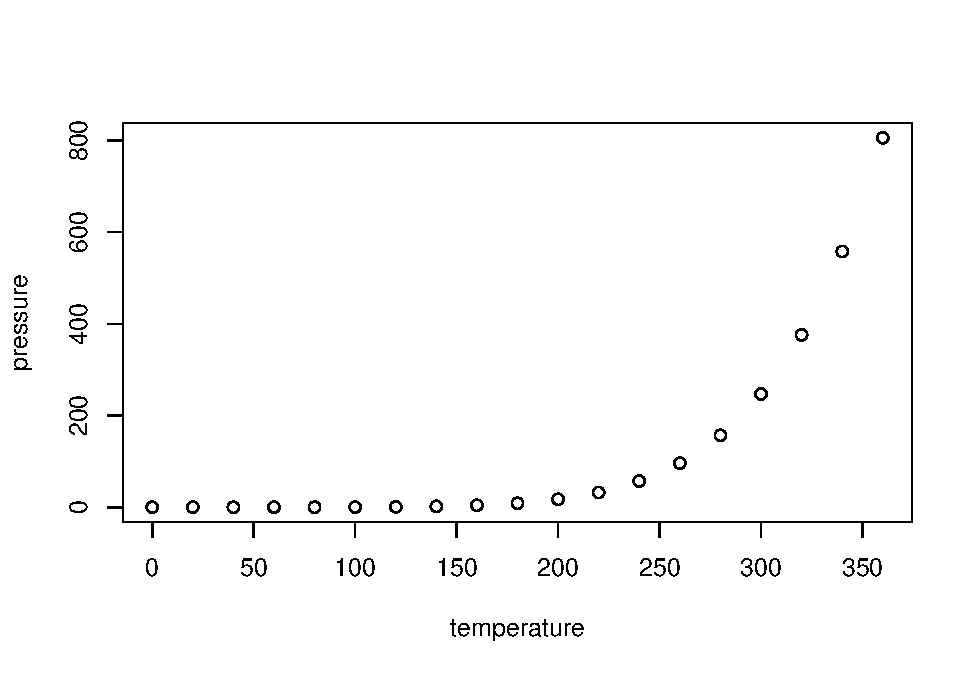
\includegraphics{Locker-Angelina-ADA-Homework-02_files/figure-latex/pressure-1.pdf}

Note that the \texttt{echo\ =\ FALSE} parameter was added to the code
chunk to prevent printing of the R code that generated the plot.

\begin{enumerate}
\def\labelenumi{\arabic{enumi}.}
\tightlist
\item
  Every Saturday, at the same time, a primatologist goes and sits in the
  forest in the morning and listens for titi monkey calls, counting the
  number of calls they hear in a 2 hour window from 5am to 7am. Based on
  previous knowledge, she believes that the mean number calls she will
  hear in that time is 15. Let X represent the appropriate Poisson
  random variable of the number of calls heard in each monitoring
  session.
\end{enumerate}

\begin{Shaded}
\begin{Highlighting}[]
\NormalTok{x <-}\StringTok{ }\DecValTok{0}\OperatorTok{:}\DecValTok{30}
\end{Highlighting}
\end{Shaded}

1.a. What is the probability that she will hear more than 8 calls during
any given session?

\begin{Shaded}
\begin{Highlighting}[]
\NormalTok{x <-}\StringTok{ }\DecValTok{0}\OperatorTok{:}\DecValTok{30}
\NormalTok{l <-}\StringTok{ }\DecValTok{15}
\NormalTok{a <-}\StringTok{ }\KeywordTok{ppois}\NormalTok{(}\DataTypeTok{q =} \DecValTok{8}\NormalTok{, }\DataTypeTok{lambda =} \DecValTok{15}\NormalTok{)}
\NormalTok{eightplus <-}\StringTok{ }\DecValTok{1}\OperatorTok{-}\NormalTok{a}
\NormalTok{eightplus}
\end{Highlighting}
\end{Shaded}

\begin{verbatim}
## [1] 0.9625535
\end{verbatim}

1.b. What is the probability that she will hear no calls in a session?

\begin{Shaded}
\begin{Highlighting}[]
\NormalTok{x <-}\StringTok{ }\DecValTok{0}\OperatorTok{:}\DecValTok{30}
\NormalTok{l <-}\StringTok{ }\DecValTok{15}
\NormalTok{b <-}\StringTok{ }\KeywordTok{ppois}\NormalTok{(}\DataTypeTok{q =} \DecValTok{0}\NormalTok{, }\DataTypeTok{lambda =} \DecValTok{15}\NormalTok{)}
\NormalTok{zero <-}\StringTok{ }\DecValTok{1}\OperatorTok{-}\NormalTok{b}
\NormalTok{zero}
\end{Highlighting}
\end{Shaded}

\begin{verbatim}
## [1] 0.9999997
\end{verbatim}

1.c. What is the probability that she will hear exactly 3 calls in a
session?

\begin{Shaded}
\begin{Highlighting}[]
\NormalTok{x <-}\StringTok{ }\DecValTok{0}\OperatorTok{:}\DecValTok{30}
\NormalTok{l <-}\StringTok{ }\DecValTok{15}
\NormalTok{c <-}\StringTok{ }\KeywordTok{dpois}\NormalTok{(}\DataTypeTok{x =} \DecValTok{3}\NormalTok{, }\DataTypeTok{lambda =} \DecValTok{15}\NormalTok{)}
\NormalTok{exactthree <-}\StringTok{ }\DecValTok{1}\OperatorTok{-}\NormalTok{c}
\NormalTok{exactthree}
\end{Highlighting}
\end{Shaded}

\begin{verbatim}
## [1] 0.9998279
\end{verbatim}

1.d. Plot the relevant Poisson mass function over the values in range 0
≤ x ≤ 30.

\begin{Shaded}
\begin{Highlighting}[]
\NormalTok{x <-}\StringTok{ }\DecValTok{0}\OperatorTok{:}\DecValTok{30}
\NormalTok{l <-}\StringTok{ }\DecValTok{15}
\NormalTok{probset <-}\StringTok{ }\KeywordTok{dpois}\NormalTok{(}\DataTypeTok{x =}\NormalTok{ x, }\DataTypeTok{lambda =}\NormalTok{ l)}
\KeywordTok{barplot}\NormalTok{(probset, }\DataTypeTok{names.arg =}\NormalTok{ x, }\DataTypeTok{space =} \DecValTok{0}\NormalTok{, }\DataTypeTok{xlab =} \StringTok{"x"}\NormalTok{, }\DataTypeTok{ylab =} \StringTok{"Pr(X = x)"}\NormalTok{, }\DataTypeTok{main =} \KeywordTok{paste0}\NormalTok{(}\StringTok{"Probability Mass Function}\CharTok{\textbackslash{}n}\StringTok{lambda = "}\NormalTok{, }\DecValTok{15}\NormalTok{))}
\end{Highlighting}
\end{Shaded}

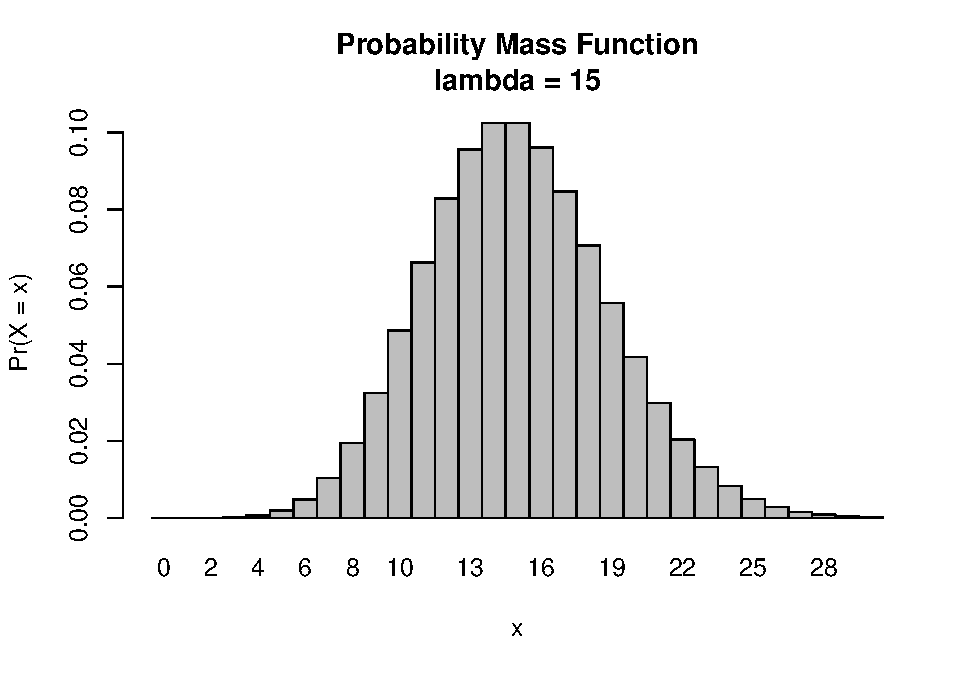
\includegraphics{Locker-Angelina-ADA-Homework-02_files/figure-latex/unnamed-chunk-5-1.pdf}

1.e. Simulate 104 results from this distribution (i.e., 2 years of
Saturday monitoring sessions).

\begin{Shaded}
\begin{Highlighting}[]
\NormalTok{x <-}\StringTok{ }\DecValTok{0}\OperatorTok{:}\DecValTok{30}
\NormalTok{l <-}\StringTok{ }\DecValTok{15}

\NormalTok{two_year <-}\StringTok{ }\KeywordTok{rpois}\NormalTok{(}\DataTypeTok{n =} \DecValTok{104}\NormalTok{, }\DataTypeTok{lambda =} \DecValTok{15}\NormalTok{)}


\NormalTok{two_year}
\end{Highlighting}
\end{Shaded}

\begin{verbatim}
##   [1] 12 10 23 14 14 16 14 15 15 12 13 17 14 13 14  6 12 13 11 13 13 12 16
##  [24] 16 14 17 19 18 12 17 17 20 16 13 16 13 16 16 16 12 21 11 11 13 16 18
##  [47] 15 12 12 10  7 15 15 19 12 16 17 10 13 16 12 20 10 16 16 19 15 13 15
##  [70] 10 13 14 10 15 14 14 11 15 13 15 26  7 19 15 18 20 17 22 14 10 16  9
##  [93] 11 21 20 15 18 14 14 12 18 13 18 12
\end{verbatim}

1.f. Plot the simulated results using hist() and use xlim() to set the
horizontal limits to be from 0 to 30. How does your histogram compare to
the shape of the probability mass function you plotted above?

\begin{Shaded}
\begin{Highlighting}[]
\NormalTok{two_year <-}\StringTok{ }\KeywordTok{rpois}\NormalTok{(}\DataTypeTok{n =} \DecValTok{104}\NormalTok{, }\DataTypeTok{lambda =} \DecValTok{15}\NormalTok{)}

\KeywordTok{hist}\NormalTok{(two_year, }\DataTypeTok{xlim=}\KeywordTok{c}\NormalTok{(}\DecValTok{0}\NormalTok{,}\DecValTok{30}\NormalTok{), }\DataTypeTok{xlab =} \StringTok{"Observation"}\NormalTok{, }\DataTypeTok{ylab =} \StringTok{"# of Calls"}\NormalTok{, }\DataTypeTok{main =} \StringTok{"# of Calls in Two Years of Observations"}\NormalTok{)}
\end{Highlighting}
\end{Shaded}

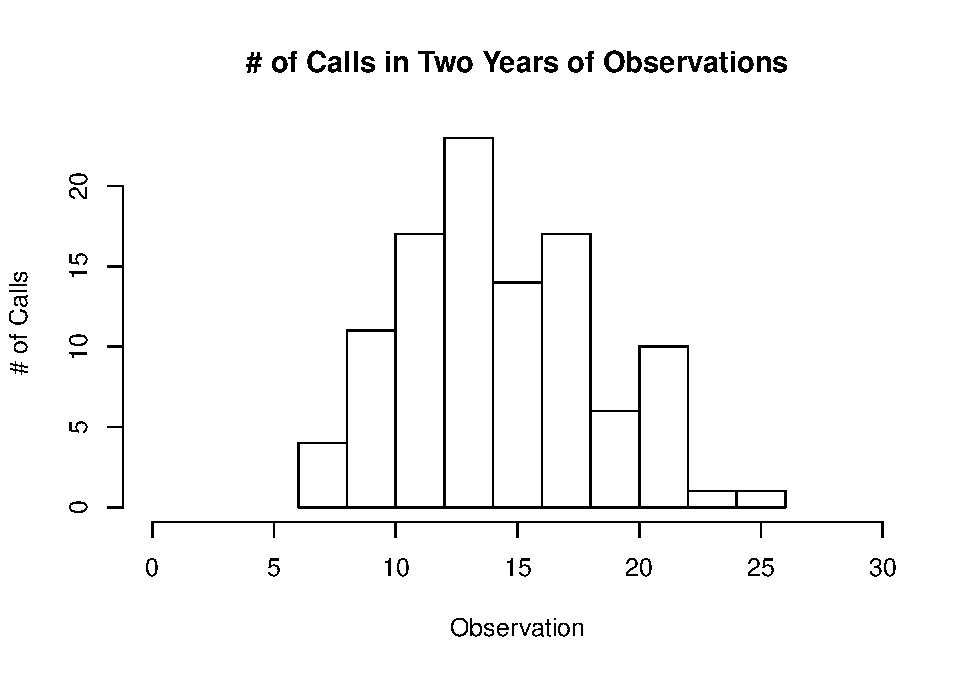
\includegraphics{Locker-Angelina-ADA-Homework-02_files/figure-latex/unnamed-chunk-7-1.pdf}

\begin{enumerate}
\def\labelenumi{\arabic{enumi}.}
\setcounter{enumi}{1}
\tightlist
\item
  Load in the dataset ``zombies.csv'' from my GitHub repository at
  \url{https://github.com/difiore/ADA-2019}. This data includes the
  first and last name and gender of the entire population of 1000 people
  who have survived the zombie apocalypse and are now ekeing out an
  existence somewhere on the East Coast, along with several other
  variables (height, weight, age, number of years of education, number
  of zombies they have killed, and college major see here for info on
  important post-zombie apocalypse majors
\end{enumerate}

\begin{Shaded}
\begin{Highlighting}[]
\KeywordTok{library}\NormalTok{(curl)}
\NormalTok{f <-}\StringTok{ }\NormalTok{f <-}\StringTok{ }\KeywordTok{curl}\NormalTok{(}\StringTok{"https://raw.githubusercontent.com/difiore/ADA-2019/master/zombies.csv"}\NormalTok{)}
\NormalTok{d <-}\StringTok{ }\KeywordTok{read.csv}\NormalTok{(f, }\DataTypeTok{header =} \OtherTok{TRUE}\NormalTok{, }\DataTypeTok{sep =} \StringTok{","}\NormalTok{, }\DataTypeTok{stringsAsFactors =} \OtherTok{FALSE}\NormalTok{)}
\KeywordTok{head}\NormalTok{(d)}
\end{Highlighting}
\end{Shaded}

\begin{verbatim}
##   id first_name last_name gender   height   weight zombies_killed
## 1  1      Sarah    Little Female 62.88951 132.0872              2
## 2  2       Mark    Duncan   Male 67.80277 146.3753              5
## 3  3    Brandon     Perez   Male 72.12908 152.9370              1
## 4  4      Roger   Coleman   Male 66.78484 129.7418              5
## 5  5      Tammy    Powell Female 64.71832 132.4265              4
## 6  6    Anthony     Green   Male 71.24326 152.5246              1
##   years_of_education                           major      age
## 1                  1                medicine/nursing 17.64275
## 2                  3 criminal justice administration 22.58951
## 3                  1                       education 21.91276
## 4                  6                  energy studies 18.19058
## 5                  3                       logistics 21.10399
## 6                  4                  energy studies 21.48355
\end{verbatim}

2.a. Calculate the population mean and standard deviation for each
quantitative random variable (height, weight, age, number of zombies
killed, and years of education). NOTE: You will not want to use the
built in var() and sd() commands as those are for samples.

\begin{Shaded}
\begin{Highlighting}[]
\KeywordTok{library}\NormalTok{(tidyverse)}
\end{Highlighting}
\end{Shaded}

\begin{verbatim}
## -- Attaching packages --------------------------------------- tidyverse 1.2.1 --
\end{verbatim}

\begin{verbatim}
## v ggplot2 3.1.0     v purrr   0.3.0
## v tibble  2.0.1     v dplyr   0.7.8
## v tidyr   0.8.2     v stringr 1.3.1
## v readr   1.3.1     v forcats 0.3.0
\end{verbatim}

\begin{verbatim}
## -- Conflicts ------------------------------------------ tidyverse_conflicts() --
## x dplyr::filter()     masks stats::filter()
## x dplyr::lag()        masks stats::lag()
## x readr::parse_date() masks curl::parse_date()
\end{verbatim}

\begin{Shaded}
\begin{Highlighting}[]
\KeywordTok{library}\NormalTok{(psych)}
\end{Highlighting}
\end{Shaded}

\begin{verbatim}
## 
## Attaching package: 'psych'
\end{verbatim}

\begin{verbatim}
## The following objects are masked from 'package:ggplot2':
## 
##     %+%, alpha
\end{verbatim}

\begin{Shaded}
\begin{Highlighting}[]
\NormalTok{sel_data <-}\StringTok{ }\KeywordTok{select}\NormalTok{(d,height, age, weight, zombies_killed, years_of_education)}

\KeywordTok{describe}\NormalTok{(sel_data)}
\end{Highlighting}
\end{Shaded}

\begin{verbatim}
##                    vars    n   mean    sd median trimmed   mad   min
## height                1 1000  67.63  4.31  67.50   67.58  4.23 54.15
## age                   2 1000  20.05  2.97  19.90   20.01  2.88 10.66
## weight                3 1000 143.91 18.40 142.89  143.71 18.08 90.29
## zombies_killed        4 1000   2.99  1.75   3.00    2.87  1.48  0.00
## years_of_education    5 1000   3.00  1.68   3.00    2.92  1.48  0.00
##                       max  range skew kurtosis   se
## height              80.53  26.38 0.08    -0.01 0.14
## age                 29.59  18.93 0.13     0.10 0.09
## weight             210.79 120.50 0.13    -0.01 0.58
## zombies_killed      11.00  11.00 0.67     0.54 0.06
## years_of_education   8.00   8.00 0.40    -0.21 0.05
\end{verbatim}

\begin{Shaded}
\begin{Highlighting}[]
\NormalTok{sd_height <-}\StringTok{ }\KeywordTok{sqrt}\NormalTok{(}\KeywordTok{sum}\NormalTok{((d}\OperatorTok{$}\NormalTok{height}\OperatorTok{-}\KeywordTok{mean}\NormalTok{(d}\OperatorTok{$}\NormalTok{height))}\OperatorTok{^}\DecValTok{2}\NormalTok{)}\OperatorTok{/}\KeywordTok{length}\NormalTok{(d}\OperatorTok{$}\NormalTok{height))}
                                                   
\NormalTok{sd_weight <-}\StringTok{ }\KeywordTok{sqrt}\NormalTok{(}\KeywordTok{sum}\NormalTok{((d}\OperatorTok{$}\NormalTok{weight}\OperatorTok{-}\KeywordTok{mean}\NormalTok{(d}\OperatorTok{$}\NormalTok{weight))}\OperatorTok{^}\DecValTok{2}\NormalTok{)}\OperatorTok{/}\KeywordTok{length}\NormalTok{(d}\OperatorTok{$}\NormalTok{weight))}

\NormalTok{sd_age <-}\StringTok{ }\KeywordTok{sqrt}\NormalTok{(}\KeywordTok{sum}\NormalTok{((d}\OperatorTok{$}\NormalTok{age}\OperatorTok{-}\KeywordTok{mean}\NormalTok{(d}\OperatorTok{$}\NormalTok{age))}\OperatorTok{^}\DecValTok{2}\NormalTok{)}\OperatorTok{/}\KeywordTok{length}\NormalTok{(d}\OperatorTok{$}\NormalTok{age))}

\NormalTok{sd_kills <-}\StringTok{ }\KeywordTok{sqrt}\NormalTok{(}\KeywordTok{sum}\NormalTok{((d}\OperatorTok{$}\NormalTok{zombies_killed}\OperatorTok{-}\KeywordTok{mean}\NormalTok{(d}\OperatorTok{$}\NormalTok{zombies_killed))}\OperatorTok{^}\DecValTok{2}\NormalTok{)}\OperatorTok{/}\KeywordTok{length}\NormalTok{(d}\OperatorTok{$}\NormalTok{zombies_killed)) }

\NormalTok{sd_edu <-}\StringTok{ }\KeywordTok{sqrt}\NormalTok{(}\KeywordTok{sum}\NormalTok{((d}\OperatorTok{$}\NormalTok{years_of_education}\OperatorTok{-}\KeywordTok{mean}\NormalTok{(d}\OperatorTok{$}\NormalTok{years_of_education))}\OperatorTok{^}\DecValTok{2}\NormalTok{)}\OperatorTok{/}\KeywordTok{length}\NormalTok{(d}\OperatorTok{$}\NormalTok{years_of_education)) }

\NormalTok{mean_height <-}\StringTok{ }\KeywordTok{mean}\NormalTok{(d}\OperatorTok{$}\NormalTok{height)}

\NormalTok{mean_weight <-}\StringTok{ }\KeywordTok{mean}\NormalTok{(d}\OperatorTok{$}\NormalTok{weight)}

\NormalTok{mean_age <-}\StringTok{ }\KeywordTok{mean}\NormalTok{(d}\OperatorTok{$}\NormalTok{age)}

\NormalTok{mean_kills <-}\StringTok{ }\KeywordTok{mean}\NormalTok{(d}\OperatorTok{$}\NormalTok{zombies_killed)}

\NormalTok{mean_edu <-}\StringTok{ }\KeywordTok{mean}\NormalTok{(d}\OperatorTok{$}\NormalTok{years_of_education)}


\NormalTok{sd_height}
\end{Highlighting}
\end{Shaded}

\begin{verbatim}
## [1] 4.30797
\end{verbatim}

\begin{Shaded}
\begin{Highlighting}[]
\NormalTok{sd_age}
\end{Highlighting}
\end{Shaded}

\begin{verbatim}
## [1] 2.963583
\end{verbatim}

\begin{Shaded}
\begin{Highlighting}[]
\NormalTok{sd_weight}
\end{Highlighting}
\end{Shaded}

\begin{verbatim}
## [1] 18.39186
\end{verbatim}

\begin{Shaded}
\begin{Highlighting}[]
\NormalTok{sd_kills}
\end{Highlighting}
\end{Shaded}

\begin{verbatim}
## [1] 1.747551
\end{verbatim}

\begin{Shaded}
\begin{Highlighting}[]
\NormalTok{sd_edu}
\end{Highlighting}
\end{Shaded}

\begin{verbatim}
## [1] 1.675704
\end{verbatim}

\begin{Shaded}
\begin{Highlighting}[]
\NormalTok{mean_height}
\end{Highlighting}
\end{Shaded}

\begin{verbatim}
## [1] 67.6301
\end{verbatim}

\begin{Shaded}
\begin{Highlighting}[]
\NormalTok{mean_age}
\end{Highlighting}
\end{Shaded}

\begin{verbatim}
## [1] 20.04696
\end{verbatim}

\begin{Shaded}
\begin{Highlighting}[]
\NormalTok{mean_weight}
\end{Highlighting}
\end{Shaded}

\begin{verbatim}
## [1] 143.9075
\end{verbatim}

\begin{Shaded}
\begin{Highlighting}[]
\NormalTok{mean_kills}
\end{Highlighting}
\end{Shaded}

\begin{verbatim}
## [1] 2.992
\end{verbatim}

\begin{Shaded}
\begin{Highlighting}[]
\NormalTok{mean_edu}
\end{Highlighting}
\end{Shaded}

\begin{verbatim}
## [1] 2.996
\end{verbatim}

2.b. Use \{ggplot\} and make boxplots of each of these variable by
gender.

\begin{Shaded}
\begin{Highlighting}[]
\KeywordTok{library}\NormalTok{(tidyverse)}
\KeywordTok{library}\NormalTok{(ggplot2)}
\NormalTok{a <-}\StringTok{ }\KeywordTok{ggplot}\NormalTok{(}\DataTypeTok{data =}\NormalTok{ d, }\KeywordTok{aes}\NormalTok{(}\DataTypeTok{x =}\NormalTok{ gender, }\DataTypeTok{y =}\NormalTok{ age, }\DataTypeTok{color =}\NormalTok{ gender)) }\OperatorTok{+}\StringTok{ }\KeywordTok{xlab}\NormalTok{(}\StringTok{"Gender"}\NormalTok{) }\OperatorTok{+}\StringTok{ }\KeywordTok{ylab}\NormalTok{(}\StringTok{"Age"}\NormalTok{) }\OperatorTok{+}\StringTok{ }\KeywordTok{geom_boxplot}\NormalTok{(}\DataTypeTok{na.rm =} \OtherTok{TRUE}\NormalTok{) }\OperatorTok{+}\StringTok{ }\KeywordTok{theme}\NormalTok{(}\DataTypeTok{legend.position =} \StringTok{"bottom"}\NormalTok{, }\DataTypeTok{legend.title =} \KeywordTok{element_blank}\NormalTok{())}
\NormalTok{a}
\end{Highlighting}
\end{Shaded}

\includegraphics{Locker-Angelina-ADA-Homework-02_files/figure-latex/unnamed-chunk-10-1.pdf}

\begin{Shaded}
\begin{Highlighting}[]
\NormalTok{w <-}\StringTok{ }\KeywordTok{ggplot}\NormalTok{(}\DataTypeTok{data =}\NormalTok{ d, }\KeywordTok{aes}\NormalTok{(}\DataTypeTok{x =}\NormalTok{ gender, }\DataTypeTok{y =}\NormalTok{ weight, }\DataTypeTok{color =}\NormalTok{ gender)) }\OperatorTok{+}\StringTok{ }\KeywordTok{xlab}\NormalTok{(}\StringTok{"Gender"}\NormalTok{) }\OperatorTok{+}\StringTok{ }\KeywordTok{ylab}\NormalTok{(}\StringTok{"Weight"}\NormalTok{) }\OperatorTok{+}\StringTok{ }\KeywordTok{geom_boxplot}\NormalTok{(}\DataTypeTok{na.rm =} \OtherTok{TRUE}\NormalTok{) }\OperatorTok{+}\StringTok{ }\KeywordTok{theme}\NormalTok{(}\DataTypeTok{legend.position =} \StringTok{"bottom"}\NormalTok{, }\DataTypeTok{legend.title =} \KeywordTok{element_blank}\NormalTok{())}
\NormalTok{w}
\end{Highlighting}
\end{Shaded}

\includegraphics{Locker-Angelina-ADA-Homework-02_files/figure-latex/unnamed-chunk-10-2.pdf}

\begin{Shaded}
\begin{Highlighting}[]
\NormalTok{h <-}\StringTok{ }\KeywordTok{ggplot}\NormalTok{(}\DataTypeTok{data =}\NormalTok{ d, }\KeywordTok{aes}\NormalTok{(}\DataTypeTok{x =}\NormalTok{ gender, }\DataTypeTok{y =}\NormalTok{ height, }\DataTypeTok{color =}\NormalTok{ gender)) }\OperatorTok{+}\StringTok{ }\KeywordTok{xlab}\NormalTok{(}\StringTok{"Gender"}\NormalTok{) }\OperatorTok{+}\StringTok{ }\KeywordTok{ylab}\NormalTok{(}\StringTok{"Height"}\NormalTok{) }\OperatorTok{+}\StringTok{ }\KeywordTok{geom_boxplot}\NormalTok{(}\DataTypeTok{na.rm =} \OtherTok{TRUE}\NormalTok{) }\OperatorTok{+}\StringTok{ }\KeywordTok{theme}\NormalTok{(}\DataTypeTok{legend.position =} \StringTok{"bottom"}\NormalTok{, }\DataTypeTok{legend.title =} \KeywordTok{element_blank}\NormalTok{())}
\NormalTok{h}
\end{Highlighting}
\end{Shaded}

\includegraphics{Locker-Angelina-ADA-Homework-02_files/figure-latex/unnamed-chunk-10-3.pdf}

\begin{Shaded}
\begin{Highlighting}[]
\NormalTok{z <-}\StringTok{ }\KeywordTok{ggplot}\NormalTok{(}\DataTypeTok{data =}\NormalTok{ d, }\KeywordTok{aes}\NormalTok{(}\DataTypeTok{x =}\NormalTok{ gender, }\DataTypeTok{y =}\NormalTok{ zombies_killed, }\DataTypeTok{color =}\NormalTok{ gender)) }\OperatorTok{+}\StringTok{ }\KeywordTok{xlab}\NormalTok{(}\StringTok{"Gender"}\NormalTok{) }\OperatorTok{+}\StringTok{ }\KeywordTok{ylab}\NormalTok{(}\StringTok{"Kills"}\NormalTok{) }\OperatorTok{+}\StringTok{ }\KeywordTok{geom_boxplot}\NormalTok{(}\DataTypeTok{na.rm =} \OtherTok{TRUE}\NormalTok{) }\OperatorTok{+}\StringTok{ }\KeywordTok{theme}\NormalTok{(}\DataTypeTok{legend.position =} \StringTok{"bottom"}\NormalTok{, }\DataTypeTok{legend.title =} \KeywordTok{element_blank}\NormalTok{())}
\NormalTok{z}
\end{Highlighting}
\end{Shaded}

\includegraphics{Locker-Angelina-ADA-Homework-02_files/figure-latex/unnamed-chunk-10-4.pdf}

\begin{Shaded}
\begin{Highlighting}[]
\NormalTok{e <-}\StringTok{ }\KeywordTok{ggplot}\NormalTok{(}\DataTypeTok{data =}\NormalTok{ d, }\KeywordTok{aes}\NormalTok{(}\DataTypeTok{x =}\NormalTok{ gender, }\DataTypeTok{y =}\NormalTok{ years_of_education, }\DataTypeTok{color =}\NormalTok{ gender)) }\OperatorTok{+}\StringTok{ }\KeywordTok{xlab}\NormalTok{(}\StringTok{"Gender"}\NormalTok{) }\OperatorTok{+}\StringTok{ }\KeywordTok{ylab}\NormalTok{(}\StringTok{"Education"}\NormalTok{) }\OperatorTok{+}\StringTok{ }\KeywordTok{geom_boxplot}\NormalTok{(}\DataTypeTok{na.rm =} \OtherTok{TRUE}\NormalTok{) }\OperatorTok{+}\StringTok{ }\KeywordTok{theme}\NormalTok{(}\DataTypeTok{legend.position =} \StringTok{"bottom"}\NormalTok{, }\DataTypeTok{legend.title =} \KeywordTok{element_blank}\NormalTok{())}
\NormalTok{e}
\end{Highlighting}
\end{Shaded}

\includegraphics{Locker-Angelina-ADA-Homework-02_files/figure-latex/unnamed-chunk-10-5.pdf}

2.c. Use \{ggplot\} and make scatterplots of height and weight in
relation to age. Do these variables seem to be related? In what way?
\emph{Both height and weight, in relation to age, have positive linear
correlations. Height and age is a stong(ish) positive linear
correlation; weight and age is a weak positive linear correlation}

\begin{Shaded}
\begin{Highlighting}[]
\NormalTok{h <-}\StringTok{ }\KeywordTok{ggplot}\NormalTok{(}\DataTypeTok{data =}\NormalTok{ d, }\KeywordTok{aes}\NormalTok{(}\DataTypeTok{x =}\NormalTok{ age, }\DataTypeTok{y =}\NormalTok{ height)) }\OperatorTok{+}\StringTok{ }\KeywordTok{xlab}\NormalTok{(}\StringTok{"Age"}\NormalTok{) }\OperatorTok{+}\StringTok{ }\KeywordTok{ylab}\NormalTok{(}\StringTok{"Height"}\NormalTok{) }\OperatorTok{+}\StringTok{ }\KeywordTok{geom_point}\NormalTok{(}\DataTypeTok{na.rm =} \OtherTok{TRUE}\NormalTok{) }\OperatorTok{+}\StringTok{ }\KeywordTok{theme}\NormalTok{(}\DataTypeTok{legend.position =} \StringTok{"bottom"}\NormalTok{, }\DataTypeTok{legend.title =} \KeywordTok{element_blank}\NormalTok{())}
\NormalTok{h}
\end{Highlighting}
\end{Shaded}

\includegraphics{Locker-Angelina-ADA-Homework-02_files/figure-latex/unnamed-chunk-11-1.pdf}

\begin{Shaded}
\begin{Highlighting}[]
\NormalTok{w <-}\StringTok{ }\KeywordTok{ggplot}\NormalTok{(}\DataTypeTok{data =}\NormalTok{ d, }\KeywordTok{aes}\NormalTok{(}\DataTypeTok{x =}\NormalTok{ age, }\DataTypeTok{y =}\NormalTok{ weight)) }\OperatorTok{+}\StringTok{ }\KeywordTok{xlab}\NormalTok{(}\StringTok{"Age"}\NormalTok{) }\OperatorTok{+}\StringTok{ }\KeywordTok{ylab}\NormalTok{(}\StringTok{"Weight"}\NormalTok{) }\OperatorTok{+}\StringTok{ }\KeywordTok{geom_point}\NormalTok{(}\DataTypeTok{na.rm =} \OtherTok{TRUE}\NormalTok{) }\OperatorTok{+}\StringTok{ }\KeywordTok{theme}\NormalTok{(}\DataTypeTok{legend.position =} \StringTok{"bottom"}\NormalTok{, }\DataTypeTok{legend.title =} \KeywordTok{element_blank}\NormalTok{())}
\NormalTok{w}
\end{Highlighting}
\end{Shaded}

\includegraphics{Locker-Angelina-ADA-Homework-02_files/figure-latex/unnamed-chunk-11-2.pdf}

2.d. Using histograms and Q-Q plots, check whether the quantitative
variables seem to be drawn from a normal distribution. Which seem to be
and which do not? \emph{Kills and Edu are not from normal distributions}

\begin{Shaded}
\begin{Highlighting}[]
\KeywordTok{hist}\NormalTok{(d}\OperatorTok{$}\NormalTok{age)}
\end{Highlighting}
\end{Shaded}

\includegraphics{Locker-Angelina-ADA-Homework-02_files/figure-latex/unnamed-chunk-12-1.pdf}

\begin{Shaded}
\begin{Highlighting}[]
\KeywordTok{hist}\NormalTok{(d}\OperatorTok{$}\NormalTok{weight)}
\end{Highlighting}
\end{Shaded}

\includegraphics{Locker-Angelina-ADA-Homework-02_files/figure-latex/unnamed-chunk-12-2.pdf}

\begin{Shaded}
\begin{Highlighting}[]
\KeywordTok{hist}\NormalTok{(d}\OperatorTok{$}\NormalTok{height)}
\end{Highlighting}
\end{Shaded}

\includegraphics{Locker-Angelina-ADA-Homework-02_files/figure-latex/unnamed-chunk-12-3.pdf}

\begin{Shaded}
\begin{Highlighting}[]
\KeywordTok{hist}\NormalTok{(d}\OperatorTok{$}\NormalTok{zombies_killed)}
\end{Highlighting}
\end{Shaded}

\includegraphics{Locker-Angelina-ADA-Homework-02_files/figure-latex/unnamed-chunk-12-4.pdf}

\begin{Shaded}
\begin{Highlighting}[]
\KeywordTok{hist}\NormalTok{(d}\OperatorTok{$}\NormalTok{years_of_education)}
\end{Highlighting}
\end{Shaded}

\includegraphics{Locker-Angelina-ADA-Homework-02_files/figure-latex/unnamed-chunk-12-5.pdf}

\begin{Shaded}
\begin{Highlighting}[]
\KeywordTok{qqnorm}\NormalTok{(d}\OperatorTok{$}\NormalTok{age, }\DataTypeTok{main =} \StringTok{"QQ Age"}\NormalTok{)}
\KeywordTok{qqline}\NormalTok{(d}\OperatorTok{$}\NormalTok{age, }\DataTypeTok{col =} \StringTok{"gray"}\NormalTok{)}
\end{Highlighting}
\end{Shaded}

\includegraphics{Locker-Angelina-ADA-Homework-02_files/figure-latex/unnamed-chunk-12-6.pdf}

\begin{Shaded}
\begin{Highlighting}[]
\KeywordTok{qqnorm}\NormalTok{(d}\OperatorTok{$}\NormalTok{weight, }\DataTypeTok{main =} \StringTok{"QQ Weight"}\NormalTok{)}
\KeywordTok{qqline}\NormalTok{(d}\OperatorTok{$}\NormalTok{weight, }\DataTypeTok{col =} \StringTok{"gray"}\NormalTok{)}
\end{Highlighting}
\end{Shaded}

\includegraphics{Locker-Angelina-ADA-Homework-02_files/figure-latex/unnamed-chunk-12-7.pdf}

\begin{Shaded}
\begin{Highlighting}[]
\KeywordTok{qqnorm}\NormalTok{(d}\OperatorTok{$}\NormalTok{height, }\DataTypeTok{main =} \StringTok{"QQ Height"}\NormalTok{)}
\KeywordTok{qqline}\NormalTok{(d}\OperatorTok{$}\NormalTok{height, }\DataTypeTok{col =} \StringTok{"gray"}\NormalTok{)}
\end{Highlighting}
\end{Shaded}

\includegraphics{Locker-Angelina-ADA-Homework-02_files/figure-latex/unnamed-chunk-12-8.pdf}

\begin{Shaded}
\begin{Highlighting}[]
\KeywordTok{qqnorm}\NormalTok{(d}\OperatorTok{$}\NormalTok{zombies_killed, }\DataTypeTok{main =} \StringTok{"QQ Kills"}\NormalTok{)}
\KeywordTok{qqline}\NormalTok{(d}\OperatorTok{$}\NormalTok{zombies_killed, }\DataTypeTok{col =} \StringTok{"gray"}\NormalTok{)}
\end{Highlighting}
\end{Shaded}

\includegraphics{Locker-Angelina-ADA-Homework-02_files/figure-latex/unnamed-chunk-12-9.pdf}

\begin{Shaded}
\begin{Highlighting}[]
\KeywordTok{qqnorm}\NormalTok{(d}\OperatorTok{$}\NormalTok{years_of_education, }\DataTypeTok{main =} \StringTok{"QQ Education"}\NormalTok{)}
\KeywordTok{qqline}\NormalTok{(d}\OperatorTok{$}\NormalTok{years_of_education, }\DataTypeTok{col =} \StringTok{"gray"}\NormalTok{)}
\end{Highlighting}
\end{Shaded}

\includegraphics{Locker-Angelina-ADA-Homework-02_files/figure-latex/unnamed-chunk-12-10.pdf}

HINT: Not all are drawn from a normal distribution! For those that are
not, can you determine what common distribution they are drawn from?

2.e. Now use the sample() function to sample ONE subset of 30 zombies
(without replacement) from this population and calculate the mean and
sample standard deviation for each variable. Also estimate the standard
error for each variable and construct the 95\% confidence interval for
each mean. Note that for the variables that are not drawn from the
normal distribution, you will need to base your estimate of the CIs on
some different distribution!

\begin{Shaded}
\begin{Highlighting}[]
\NormalTok{variables <-}\StringTok{ }
\NormalTok{k <-}\StringTok{ }\DecValTok{1}  \CommentTok{# number of subsets taken}
\NormalTok{n <-}\StringTok{ }\DecValTok{30}  \CommentTok{# subset size}
\NormalTok{age <-}\StringTok{ }\OtherTok{NULL} \CommentTok{# dummy}
\ControlFlowTok{for}\NormalTok{ (i }\ControlFlowTok{in} \DecValTok{1}\OperatorTok{:}\NormalTok{k) \{}
\NormalTok{  age[[i]] <-}\StringTok{ }\KeywordTok{sample}\NormalTok{(d}\OperatorTok{$}\NormalTok{age, }\DataTypeTok{size =}\NormalTok{ n, }\DataTypeTok{replace =} \OtherTok{FALSE}\NormalTok{)}
\NormalTok{\}}

\KeywordTok{head}\NormalTok{(age)}
\end{Highlighting}
\end{Shaded}

\begin{verbatim}
## [[1]]
##  [1] 18.87523 18.84754 19.73432 22.01716 25.83258 20.98309 29.17945
##  [8] 22.99593 16.54507 16.56274 23.86443 18.13684 21.16551 18.06575
## [15] 22.67476 18.32146 20.37872 21.12570 17.01380 19.27299 20.93505
## [22] 16.81380 16.65884 16.17854 17.92773 18.62649 18.23132 19.58134
## [29] 19.57079 17.09370
\end{verbatim}

\begin{Shaded}
\begin{Highlighting}[]
\NormalTok{mage <-}\StringTok{ }\KeywordTok{mean}\NormalTok{(age[[i]])}

\NormalTok{mage}
\end{Highlighting}
\end{Shaded}

\begin{verbatim}
## [1] 19.77369
\end{verbatim}

2.f. Now draw 99 more random samples of 30 zombies out and calculate the
mean for each of the these samples. Together with the first sample you
drew out, you now have a set of 100 means for each variable (each based
on 30 observations), which constitutes a sampling distribution for each
variable. What are the means and standard deviations of the sampling
distribution for each variable? How do the standard deviations compare
to the standard errors estimated in {[}2.e.{]}? What do these sampling
distributions look like? Are they normally distributed? What about for
those variables that you concluded were not originally drawn from a
normal distribution?

\begin{Shaded}
\begin{Highlighting}[]
\NormalTok{k <-}\StringTok{ }\DecValTok{99}  \CommentTok{# number of subsets taken}
\NormalTok{n <-}\StringTok{ }\DecValTok{30}  \CommentTok{# subset size}
\NormalTok{age2 <-}\StringTok{ }\OtherTok{NULL}  \CommentTok{# dummy}
\ControlFlowTok{for}\NormalTok{ (i }\ControlFlowTok{in} \DecValTok{1}\OperatorTok{:}\NormalTok{k) \{}
\NormalTok{    age2[[i]] <-}\StringTok{ }\KeywordTok{sample}\NormalTok{(d}\OperatorTok{$}\NormalTok{age, }\DataTypeTok{size =}\NormalTok{ n, }\DataTypeTok{replace =} \OtherTok{FALSE}\NormalTok{)}
\NormalTok{\}}

\KeywordTok{head}\NormalTok{(age2)}
\end{Highlighting}
\end{Shaded}

\begin{verbatim}
## [[1]]
##  [1] 20.90986 15.49664 19.58831 22.39601 22.03788 18.77472 19.19450
##  [8] 20.28010 24.98712 19.74716 21.09164 17.35896 12.29306 17.31604
## [15] 20.55057 16.33405 16.19003 26.25881 14.84844 22.34703 17.79204
## [22] 21.54377 21.80380 19.11892 22.99733 21.43846 20.90615 20.84825
## [29] 22.04910 22.84620
## 
## [[2]]
##  [1] 23.76366 14.98345 21.71185 24.01948 22.19631 27.68187 20.69956
##  [8] 21.64507 15.77083 19.16099 24.56925 18.82747 18.62649 18.99893
## [15] 26.52334 21.91309 16.19753 19.53526 17.35896 21.24646 19.37270
## [22] 22.29698 18.81568 20.35543 22.15048 21.98378 15.49664 11.13065
## [29] 15.22140 18.09670
## 
## [[3]]
##  [1] 19.81533 17.64131 21.93743 21.93253 19.36259 25.42632 19.75214
##  [8] 22.51602 20.77667 20.40242 18.54973 19.16468 20.48590 22.39316
## [15] 19.19267 21.43846 23.89309 20.26560 25.32669 18.37246 20.32666
## [22] 23.68478 22.29698 18.61992 15.96942 16.52151 22.42920 18.04177
## [29] 21.31904 17.64006
## 
## [[4]]
##  [1] 20.49434 18.58842 20.32666 24.09405 17.95730 16.15942 19.16468
##  [8] 25.32669 19.66843 21.73021 19.73432 15.44328 20.35923 20.69956
## [15] 16.40678 20.05336 23.19955 20.46354 25.11161 17.95568 18.77472
## [22] 21.42676 21.33236 18.72847 21.61279 19.38947 23.88692 18.87523
## [29] 21.43846 24.00647
## 
## [[5]]
##  [1] 18.61760 20.22591 23.97528 25.82221 22.18075 17.90380 16.62255
##  [8] 22.15048 16.75516 20.29005 18.45236 17.38376 17.08913 17.63057
## [15] 22.00580 19.55997 16.74267 20.43760 18.61704 18.43727 18.73962
## [22] 20.95489 13.12491 19.91412 20.79042 19.85983 19.59841 19.24192
## [29] 18.92719 21.64507
## 
## [[6]]
##  [1] 20.37958 16.10785 23.76366 17.95730 20.16242 21.91993 23.68478
##  [8] 19.07924 17.96982 18.89775 16.50640 20.11425 16.32636 19.87259
## [15] 20.79042 22.34368 19.16099 20.22591 23.25794 20.57065 18.67945
## [22] 17.64006 23.94809 25.57398 21.97010 18.29770 18.54973 15.47891
## [29] 23.67717 21.83863
\end{verbatim}

\begin{Shaded}
\begin{Highlighting}[]
\NormalTok{mage2 <-}\StringTok{ }\KeywordTok{mean}\NormalTok{(age2[[i]])}
\NormalTok{mage2}
\end{Highlighting}
\end{Shaded}

\begin{verbatim}
## [1] 20.38096
\end{verbatim}

\begin{Shaded}
\begin{Highlighting}[]
\NormalTok{mtage <-}\StringTok{ }\NormalTok{(mage }\OperatorTok{+}\StringTok{ }\NormalTok{mage2)}\OperatorTok{/}\DecValTok{2}
\NormalTok{mtage}
\end{Highlighting}
\end{Shaded}

\begin{verbatim}
## [1] 20.07732
\end{verbatim}

When you are done, ``knit'' your R Markdown file to .html and push both
your .Rmd and .html files up to GitHub for me to look at.


\end{document}
